\section{Ergebnisse}

\todoAll{Ergebnisse (wertungsfrei) beschreiben}

Unsere Studie wurde vom 04. Juni bis zum 18. August 2019 durchgeführt. Es nahmen insgesamt 45 Teilnehmer in zwei Durchläufen teil. Der erste Durchlauf erfasste zwei Gruppen, dessen geänderter Parameter die Zeit war in der ein Licht innerhalb der virtuellen Umgebung sie 'geweckt' hat. Im zweiten durchlauf wurde dieser Parameter geändert und die Teilnehmer wurden mit einem Ton geweckt, wie man ihn als Hinweiston in modernen Autos wiederfindet. Hierbei wurde die Zeit gemessen in der die Studienteilnehmer den Ton selbständig abgeschaltet haben. 

Es waren von den 45 Teilnehmern nach eigenen Angaben 12 weiblich, 33 männlich und 0 Divers. Eine grafische Repräsentation kann in Bild~\ref{fig:gender} und die zugehörigen Zahlenwerte in Tabelle~\ref{tab:sc_results_gender} gesehen werden. 

\begin{figure}
	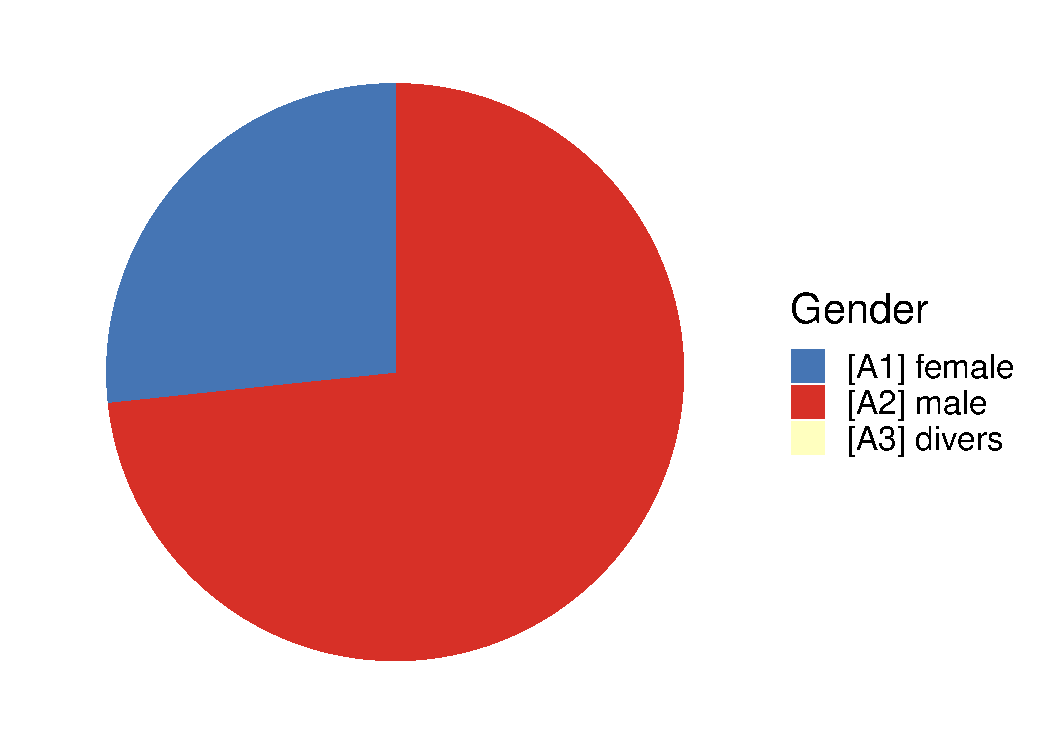
\includegraphics[width=\textwidth]{./appendices/gender}
	\caption{Geschlechterverteilung der Studienteilnehmer}
	\label{fig:gender}
\end{figure}

Das Alter der Teilnehmer reichte von 19 bis 30 Jahren, wobei der Median bei 23 und der Mittelwert bei 23,04 Jahren lag mit einer Standardabweichung von 2.53. Eine grafische Darstellung kann in Bild~\ref{fig:age} und die zugehörigen Zahlenwerte in Tabelle~\ref{tab:sc_results_age} gesehen werden.

\begin{figure}
	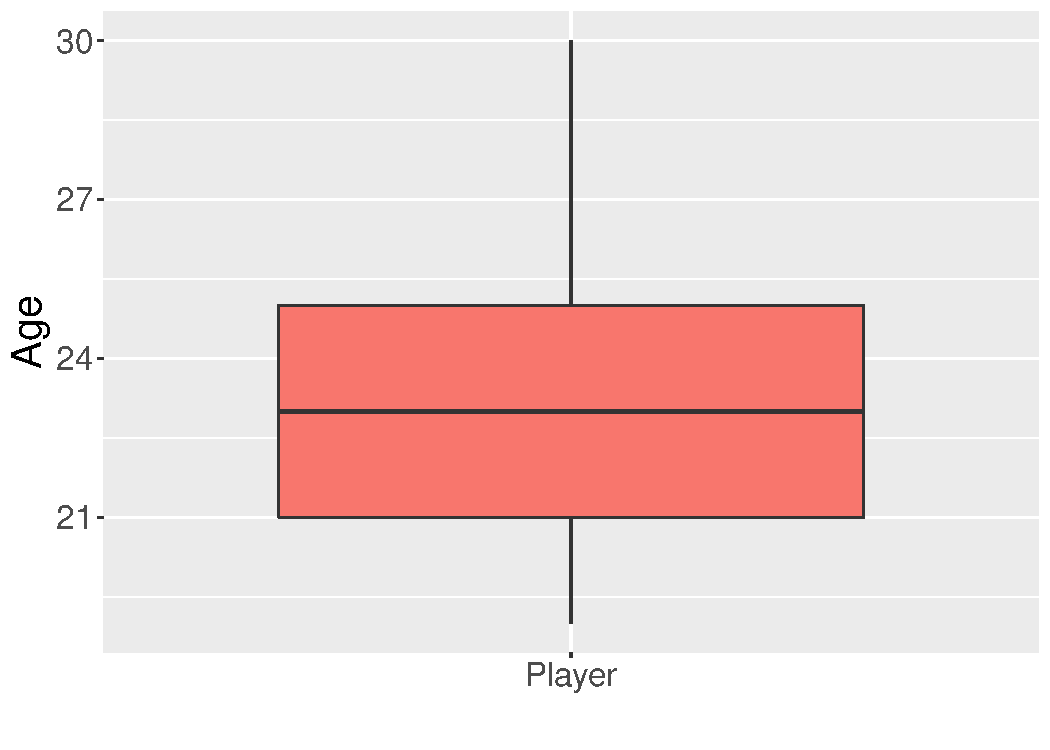
\includegraphics[width=\textwidth]{./appendices/age}
	\caption{Boxplot des Alters der Studienteilnehmer}
	\label{fig:age}
\end{figure}

Die Teilnehmer gaben an, dass sie unterdurchschnittlich wenig Erfahrung mit virtueller Realität haben. Hierbei lag der Mittelwert bei 2,93 von 7 möglichen Punkten. Die Standardabweichung beträgt 1,78. Die Ergebnisse können auch in Tabelle~\ref{tab:sc_results_expVR} und Tabelle~\ref{tab:sc_numbers_expVR} angesehen werden. Bei augmentierter Realität sehen wir ein ähnliches Bild. Hier gaben die Teilnehmer an einen durchschnittlichen Erfahrungswert von 2.36 von 7 zu haben. Die Standardabweichung in diesem Fall beträgt 1,38. Außerdem ist noch hervorzuheben, dass keiner der Befragten einen Wert von 7 ausgewählt hat. Die Ergebnisse hierzu können in Tabelle~\ref{tab:sc_results_expAR} und Tabelle~\ref{tab:sc_numbers_expAR} eingesehen werden, zusätzlich existiert eine grafische Repräsentation in den Bildern~\ref{fig:expVr} und~\ref{fig:expAr}.

\begin{figure}
	% \centering
	\begin{subfigure}{0.48\textwidth}
		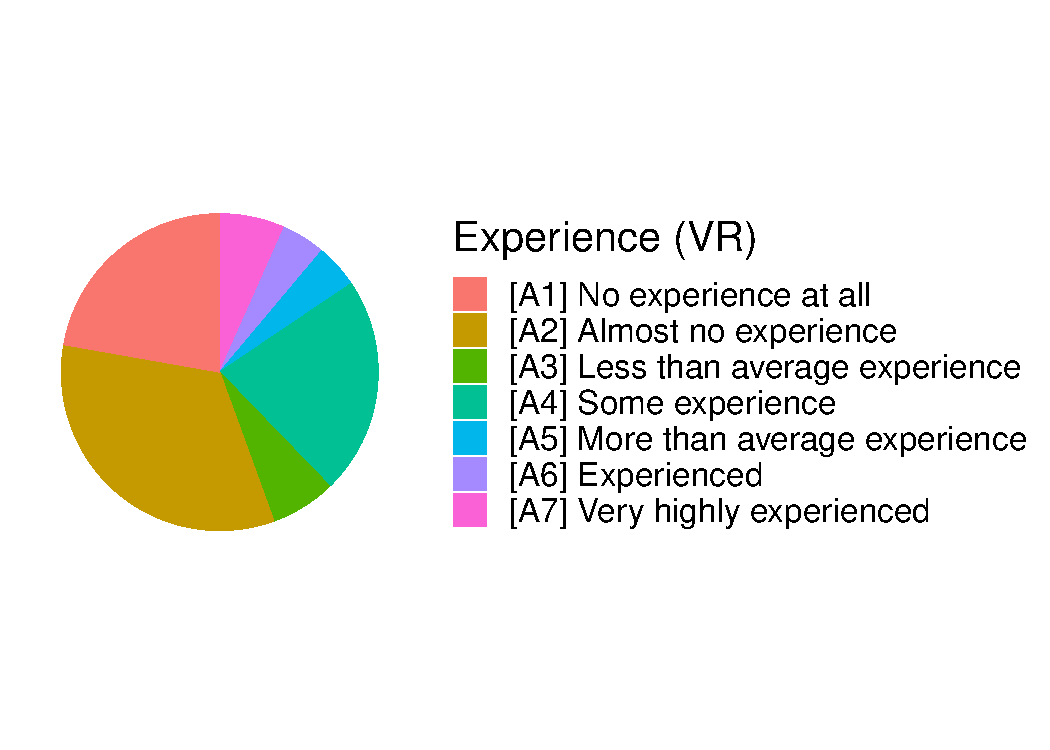
\includegraphics[width=\textwidth]{./appendices/expVr}
		\caption{Grafische Repräsentation der Antworten zur Frage 'How much experience do you have with VR?'.}
		\label{fig:expVr}
	\end{subfigure}%
	\hfill
	\begin{subfigure}{0.48\textwidth}
		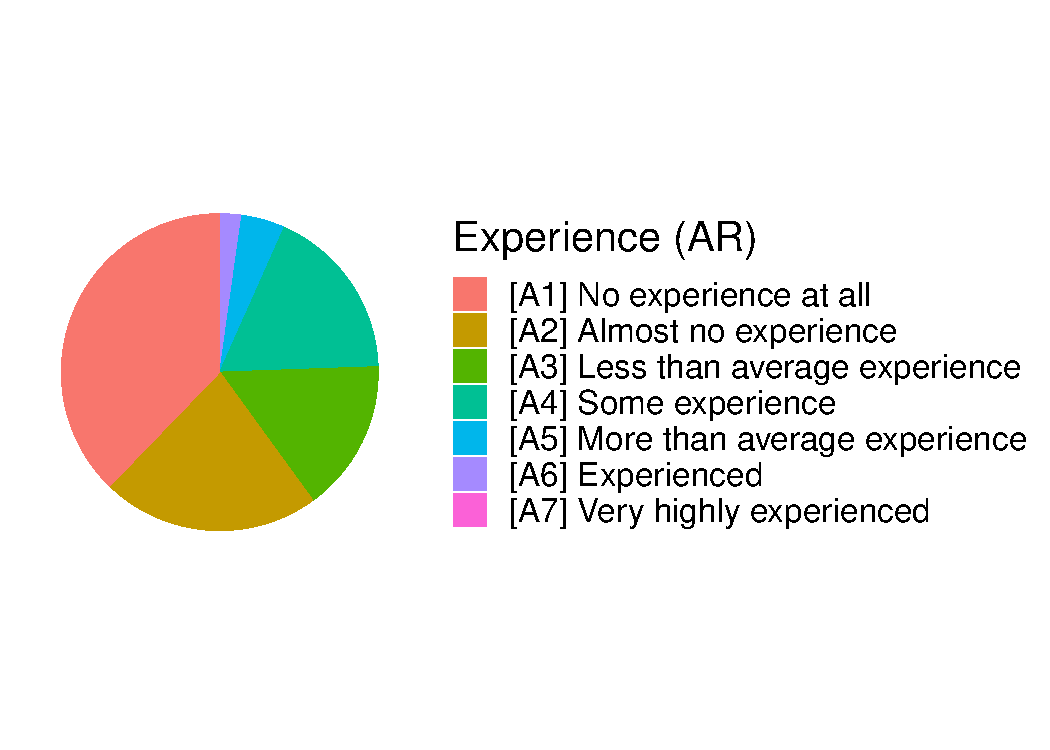
\includegraphics[width=\textwidth]{./appendices/expAr}
		\caption{Grafische Repräsentation der Antworten zur Frage 'How much experience do you have with AR?'.}
		\label{fig:expAr}
	\end{subfigure}
	\caption{Erfahrungen mit virtueller und augmentierter Realität der Studienteilnehmer}
\end{figure}

\todoTob{Mehr Ergebnisse einfügen}

\begin{figure}
	% \centering
	\begin{subfigure}{0.48\textwidth}
		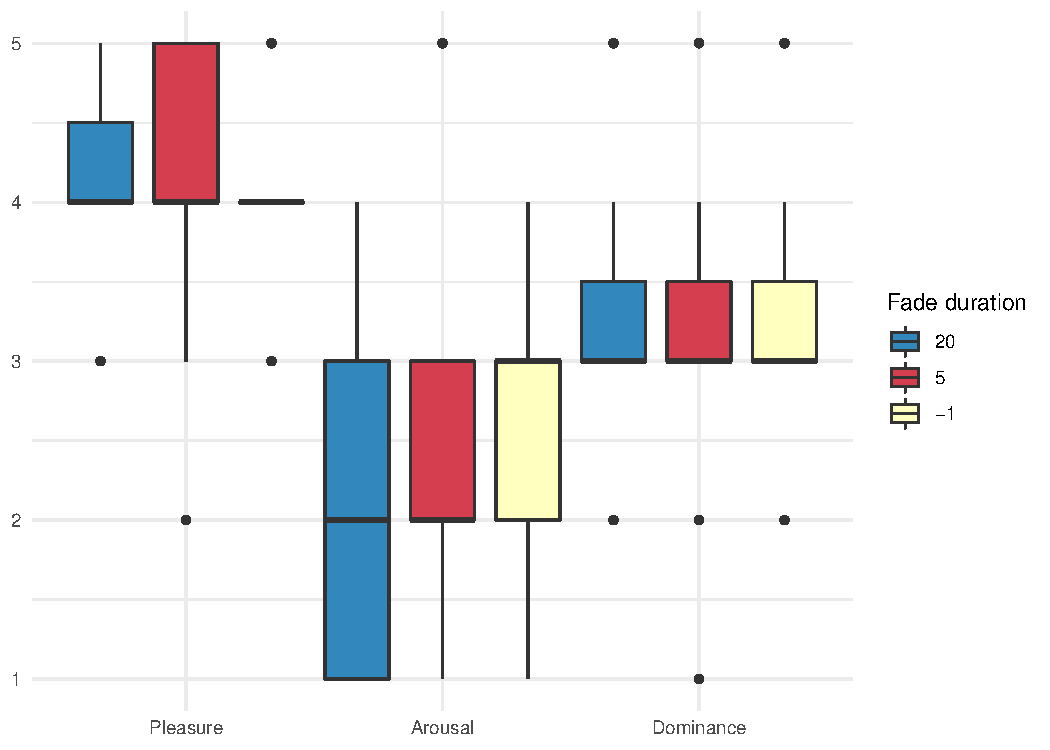
\includegraphics[width=\textwidth]{./appendices/SAMpre}
		\caption{Self-Assessment Manikin Ergebnisse vor der `Schlafphase'}
		\label{fig:samPre}
	\end{subfigure}%
	\hfill
	\begin{subfigure}{0.48\textwidth}
		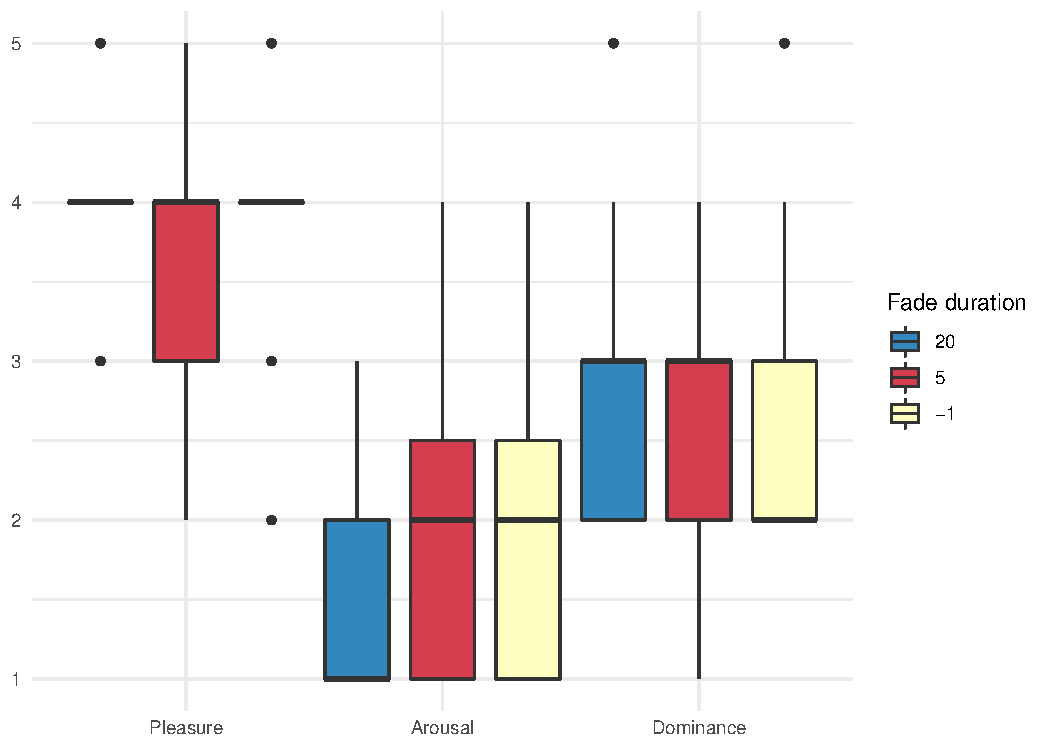
\includegraphics[width=\textwidth]{./appendices/SAMpost}
		\caption{Self-Assessment Manikin Ergebnisse nach der `Schlafphase'}
		\label{fig:samPost}
	\end{subfigure}
	\caption{Die Ergebnisse der Selbsteinschätzung zum Self-Assessment Manikin} % caption for whole figure
\end{figure}
\todoAll{Wie ist das wording für die Schlafphase?? -> ändern}
